\documentclass[12pt,letterpaper]{article}
\usepackage[top=2cm,left=2cm,right=2cm,bottom=2cm]{geometry}
\usepackage[utf8]{inputenc}
\usepackage[T1]{fontenc}  
\usepackage{ae}               % Fonte "Almost European"
\usepackage{amsmath,amssymb}
\usepackage{setspace}
\usepackage{graphicx}
\usepackage{indentfirst}
\usepackage{url}
\usepackage{color}
\usepackage{cite}
\usepackage{gensymb}
\usepackage{subcaption}
\usepackage{hyperref}
\usepackage{epigraph}
\usepackage{mathtools}
\usepackage{mathrsfs}
\usepackage{epstopdf}

\definecolor{red}{rgb}{1.0,0.0,0.0}
\definecolor{green}{rgb}{0.01,0.75,0.24}
\definecolor{blue}{rgb}{0.0,0.0,1.0}

\newcommand{\ket}[1]{| #1 \rangle}
\newcommand{\bra}[1]{\langle #1 |}
\newcommand{\expected}[1]{ \langle #1 \rangle}
\newcommand{\product}[2]{\langle #1 | #2 \rangle}
\newcommand{\pib}{\boldsymbol{\pi}}
\newcommand{\sigmab}{\boldsymbol{\sigma}}
\newcommand{\taub}{\boldsymbol{\tau}}
\newcommand{\kdotx}{\textbf{k}\cdot\textbf{x}} % k dot x

\newcommand{\project}{\large Progress Report \vskip 0.1cm}
\newcommand{\asu}{Physics Department \\ Arizona State University}

\begin{document}
\onehalfspacing
%\doublespace
\title{\project {\Large \textbf{Quantum Monte Carlo Calculations of Nucleon 
Systems and Cold Atom Gases}} \vspace{-0.5cm}}
\author{
{\bf PIs: Kevin E. Schmidt}, Arizona State University \\
{\bf Stefano Gandolfi}, Los Alamos National Laboratory
}
\date{\today}
\maketitle

\vspace{-1.5cm}
\section*{Abstract}

We present our progress on the projects we have been developing. In our study 
of strongly interacting Fermi gases, we investigated core structure properties 
of two-dimensional Fermi gas vortices
in the BEC-BCS crossover region. The manuscript with our findings is currently 
under review by Physical Review A journal. Also, we have been developing light 
nuclei wave functions which include explicit pion contributions. In our study 
of improved trial wave functions for nucleon systems, we have results for 
$^4$He, $^{16}$O, and symmetric nuclear matter.

\section{Scientific discoveries}%and accomplishments of the computational plan}

\subsection{Strongly paired fermionic systems of cold atoms}

Our findings regarding cold gases systems were summarized in the article
``Core structure of two-dimensional Fermi gas vortices
in the BEC-BCS crossover region" \cite{mad17}, which has been submitted to the 
Physical 
Review A journal.

We reported $T=0$ diffusion Monte Carlo results for 
the ground-state and vortex excitation of unpolarized spin-1/2 fermions 
in a two-dimensional disk. We investigated how vortex core structure 
properties behave over the BEC-BCS crossover. We calculated the vortex 
excitation energy, density profiles, and vortex core properties related 
to the current. We found a density suppression at the vortex core on 
the BCS side of the crossover, and a depleted core on the BEC limit. 
Size-effect dependencies in the disk geometry were carefully studied.


\subsection{QMC simulations with explicit contributions from the pion field}

We begun our study of explicit contributions of the pion field to QMC 
simulations by studying one nucleon in a box.
As a starting point,
we can try to determine the self energy (effective mass) of a nucleon of bare 
mass $m_b$, which should be equal to its physical mass. Since we consider 
dynamical pions, we are effectively including processes like the ones in 
Fig.~\ref{fig:feynman}.

\begin{figure}[!htb]
\centering
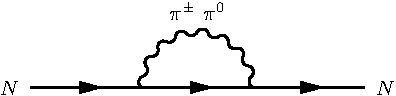
\includegraphics[width=0.6\linewidth]{feynman.pdf}
\caption{}
\label{fig:feynman}
\end{figure}
The corresponding Hamiltonian can be written as
\begin{flalign}
\hat{H} &= \sum_{k=0}^{k_c} \left\{ 
-\frac{1}{2} \nabla_{\pi_{k_\beta}^c}^2
-\frac{1}{2} \nabla_{\pi_{k_\beta}^s}^2
+\frac{1}{2}(k^2+m_\pi^2)(\pi_{k_\beta}^{c2}+\pi_{k_\beta}^{s2})
\right\} \nonumber \\
&+ \frac{g_a}{2 f_\pi} \frac{1}{\sqrt{2\pi}} \sum_{\alpha,
\beta}\sum_{k=0}^{k_c} \sigma_\alpha \tau_\beta (k_\alpha \pi_{k\beta}^s 
\cos(\kdotx) - k_\alpha \pi_{k\beta}^c \sin(\kdotx)) %\nonumber \\
 + \frac{p_i^2}{2m_b} + m_b',
\end{flalign}
where $\textbf{k}$ are wave vectors compatible with the simulation box, $k_c$ 
is a cutoff, 
$\pi_{\textbf{k}}$ are pionic degrees of freedom, $m_\pi$ is the pion mass,
$g_a$ and $f_\pi$ are coupling constants, $\textbf{x}$ are the spatial 
coordinates of the nucleon, $\sigmab$ and $\taub$ are the usual Pauli matrices 
which act on spin and isospin, respectively, and 
$\textbf{p}$ is the momentum of the nucleon.

The trial wave function which we developed is
\begin{flalign}
&\psi_T(\pib_{\textbf{k}}^c,\pib_{\textbf{k}}^s,\textbf{x})= \prod_{k=0}^{k_c} 
\exp \left[ - \sqrt{k^2+m_\pi^2} \left\{
\pib_{k_\beta}^{c2}+\pib_{k_\beta}^{s2} + \tilde{G}_k \textbf{k}\cdot\sigmab 
\left[
-\sin(\kdotx) \pib_{\textbf{k}}^c \cdot \taub \right.\right.\right. \nonumber 
\\
&\left.\left.\left. + \cos(\kdotx) \pib_{k_\beta}^{s} \cdot \taub \right]
+\tilde{G}_k^2 (\sigmab\cdot\textbf{k})^2 \taub^2 \right\} \right]
\phi
\end{flalign}
where the $\tilde{G}_k$ are variational parameters and
\begin{displaymath}
    \phi = 
    \left(
        \begin{matrix} 
        		\phi^{p\uparrow}\\
            \phi^{p\downarrow}\\
            \phi^{n\uparrow}\\
            \phi^{n\downarrow}
        \end{matrix}   
	\right)
\end{displaymath}
is a 4-spinor.
\vspace{-0.5cm}
\subsection{Improved trial wave functions for nuclei and nuclear matter}
Auxiliary Field Diffusion Monte Carlo (AFDMC) calculations depend heavily on 
having a good estimate to the ground-state wave function of the system. This 
estimate is called the trial wave function. The ideal set of spin-isospin 
dependent correlations are an exponential of spin-isospin operators. In the 
past this exponential was expanded and truncated at linear correlations 
\cite{gan14}. We have expanded the trial wave function to include quadratic 
correlations. The addition of these correlations has lowered the energies for 
each system that we have calculated compared to the same calculation with 
linear correlations. We have currently done correlations for the nuclei $^4$He 
and $^{16}$O, and for symmetric nuclear matter. Our preliminary results are summarized in Tab.~\ref{tab:indpairresults}. We have also calculated the energy per nucleon of symmetric nuclear matter (SNM) with density $\rho=0.16$fm$^{-3}$ of 28 particles with periodic boundary conditions. The energy per nucleon was -13.92(6) MeV for linear correlations, -14.80(7) MeV for independent pair correlations, and -14.70(11) MeV with the full set of quadratic correlations.

\begin{table}[h!]
   \centering
   \caption{Energy in MeV for $^4$He and $^{16}$O as calculated with all three types of correlations compared to experimental energies.}
   \label{tab:indpairresults}
   \begin{tabular}{ccccc}
      \hline \hline
       & Linear & Independent Pair & Quadratic & Experimental\\
      \hline
      $^4$He & -27.17(4) & -26.33(3) & -25.35(3) & -28.295\\
      $^{16}$O & -115.7(9) & -121.5(1.5) & -120.0(1.4) & -127.619\\
      \hline \hline
   \end{tabular}
\end{table}

It would be beneficial to include the full exponential correlations in the 
trial wave function if possible. To propagate the positions and spins of the 
configurations of particles we use a Green's function or propagator. The 
propagator involves the exponential of the Hamiltonian, which contains the same 
spin-isospin dependent operators as the wave function correlations. Currently 
the spin-isospin dependent propagator is calculated with the aid of the 
Hubbard-Stratanovich transformation as described in \cite{car15}. We plan to 
use the Hubbard-Stratanovich transformation to calculate the full exponential 
correlation operator. This should improve the trial wave function even further 
than the quadratic correlations.

With this improved trial wave function we will investigate the clustering of 
two neutrons and two protons into alpha particles in mostly neutron matter. 
Alpha particle clustering has been investigated and has shown a dependence on 
density in mostly nuclear matter \cite{sch13}. We plan to show that AFDMC is a 
viable tool to investigate this clustering.
\vspace{-0.5cm}
\section{Scientific production}
Our findings regarding cold gases systems were summarized in the article
``Core structure of two-dimensional Fermi gas vortices
in the BEC-BCS crossover region" \cite{mad17}, which is under review by the 
Physical 
Review A journal.

\vspace{-0.5cm}
%\newpage
\bibliographystyle{unsrt}
\bibliography{xsede}
\end{document}